% Options for packages loaded elsewhere
\PassOptionsToPackage{unicode}{hyperref}
\PassOptionsToPackage{hyphens}{url}
\PassOptionsToPackage{dvipsnames,svgnames,x11names}{xcolor}
%
\documentclass[
]{article}

\usepackage{amsmath,amssymb}
\usepackage{iftex}
\ifPDFTeX
  \usepackage[T1]{fontenc}
  \usepackage[utf8]{inputenc}
  \usepackage{textcomp} % provide euro and other symbols
\else % if luatex or xetex
  \usepackage{unicode-math}
  \defaultfontfeatures{Scale=MatchLowercase}
  \defaultfontfeatures[\rmfamily]{Ligatures=TeX,Scale=1}
\fi
\usepackage{lmodern}
\ifPDFTeX\else  
    % xetex/luatex font selection
\fi
% Use upquote if available, for straight quotes in verbatim environments
\IfFileExists{upquote.sty}{\usepackage{upquote}}{}
\IfFileExists{microtype.sty}{% use microtype if available
  \usepackage[]{microtype}
  \UseMicrotypeSet[protrusion]{basicmath} % disable protrusion for tt fonts
}{}
\makeatletter
\@ifundefined{KOMAClassName}{% if non-KOMA class
  \IfFileExists{parskip.sty}{%
    \usepackage{parskip}
  }{% else
    \setlength{\parindent}{0pt}
    \setlength{\parskip}{6pt plus 2pt minus 1pt}}
}{% if KOMA class
  \KOMAoptions{parskip=half}}
\makeatother
\usepackage{xcolor}
\usepackage[margin=1in]{geometry}
\setlength{\emergencystretch}{3em} % prevent overfull lines
\setcounter{secnumdepth}{5}
% Make \paragraph and \subparagraph free-standing
\makeatletter
\ifx\paragraph\undefined\else
  \let\oldparagraph\paragraph
  \renewcommand{\paragraph}{
    \@ifstar
      \xxxParagraphStar
      \xxxParagraphNoStar
  }
  \newcommand{\xxxParagraphStar}[1]{\oldparagraph*{#1}\mbox{}}
  \newcommand{\xxxParagraphNoStar}[1]{\oldparagraph{#1}\mbox{}}
\fi
\ifx\subparagraph\undefined\else
  \let\oldsubparagraph\subparagraph
  \renewcommand{\subparagraph}{
    \@ifstar
      \xxxSubParagraphStar
      \xxxSubParagraphNoStar
  }
  \newcommand{\xxxSubParagraphStar}[1]{\oldsubparagraph*{#1}\mbox{}}
  \newcommand{\xxxSubParagraphNoStar}[1]{\oldsubparagraph{#1}\mbox{}}
\fi
\makeatother

\usepackage{color}
\usepackage{fancyvrb}
\newcommand{\VerbBar}{|}
\newcommand{\VERB}{\Verb[commandchars=\\\{\}]}
\DefineVerbatimEnvironment{Highlighting}{Verbatim}{commandchars=\\\{\}}
% Add ',fontsize=\small' for more characters per line
\usepackage{framed}
\definecolor{shadecolor}{RGB}{241,243,245}
\newenvironment{Shaded}{\begin{snugshade}}{\end{snugshade}}
\newcommand{\AlertTok}[1]{\textcolor[rgb]{0.68,0.00,0.00}{#1}}
\newcommand{\AnnotationTok}[1]{\textcolor[rgb]{0.37,0.37,0.37}{#1}}
\newcommand{\AttributeTok}[1]{\textcolor[rgb]{0.40,0.45,0.13}{#1}}
\newcommand{\BaseNTok}[1]{\textcolor[rgb]{0.68,0.00,0.00}{#1}}
\newcommand{\BuiltInTok}[1]{\textcolor[rgb]{0.00,0.23,0.31}{#1}}
\newcommand{\CharTok}[1]{\textcolor[rgb]{0.13,0.47,0.30}{#1}}
\newcommand{\CommentTok}[1]{\textcolor[rgb]{0.37,0.37,0.37}{#1}}
\newcommand{\CommentVarTok}[1]{\textcolor[rgb]{0.37,0.37,0.37}{\textit{#1}}}
\newcommand{\ConstantTok}[1]{\textcolor[rgb]{0.56,0.35,0.01}{#1}}
\newcommand{\ControlFlowTok}[1]{\textcolor[rgb]{0.00,0.23,0.31}{\textbf{#1}}}
\newcommand{\DataTypeTok}[1]{\textcolor[rgb]{0.68,0.00,0.00}{#1}}
\newcommand{\DecValTok}[1]{\textcolor[rgb]{0.68,0.00,0.00}{#1}}
\newcommand{\DocumentationTok}[1]{\textcolor[rgb]{0.37,0.37,0.37}{\textit{#1}}}
\newcommand{\ErrorTok}[1]{\textcolor[rgb]{0.68,0.00,0.00}{#1}}
\newcommand{\ExtensionTok}[1]{\textcolor[rgb]{0.00,0.23,0.31}{#1}}
\newcommand{\FloatTok}[1]{\textcolor[rgb]{0.68,0.00,0.00}{#1}}
\newcommand{\FunctionTok}[1]{\textcolor[rgb]{0.28,0.35,0.67}{#1}}
\newcommand{\ImportTok}[1]{\textcolor[rgb]{0.00,0.46,0.62}{#1}}
\newcommand{\InformationTok}[1]{\textcolor[rgb]{0.37,0.37,0.37}{#1}}
\newcommand{\KeywordTok}[1]{\textcolor[rgb]{0.00,0.23,0.31}{\textbf{#1}}}
\newcommand{\NormalTok}[1]{\textcolor[rgb]{0.00,0.23,0.31}{#1}}
\newcommand{\OperatorTok}[1]{\textcolor[rgb]{0.37,0.37,0.37}{#1}}
\newcommand{\OtherTok}[1]{\textcolor[rgb]{0.00,0.23,0.31}{#1}}
\newcommand{\PreprocessorTok}[1]{\textcolor[rgb]{0.68,0.00,0.00}{#1}}
\newcommand{\RegionMarkerTok}[1]{\textcolor[rgb]{0.00,0.23,0.31}{#1}}
\newcommand{\SpecialCharTok}[1]{\textcolor[rgb]{0.37,0.37,0.37}{#1}}
\newcommand{\SpecialStringTok}[1]{\textcolor[rgb]{0.13,0.47,0.30}{#1}}
\newcommand{\StringTok}[1]{\textcolor[rgb]{0.13,0.47,0.30}{#1}}
\newcommand{\VariableTok}[1]{\textcolor[rgb]{0.07,0.07,0.07}{#1}}
\newcommand{\VerbatimStringTok}[1]{\textcolor[rgb]{0.13,0.47,0.30}{#1}}
\newcommand{\WarningTok}[1]{\textcolor[rgb]{0.37,0.37,0.37}{\textit{#1}}}

\providecommand{\tightlist}{%
  \setlength{\itemsep}{0pt}\setlength{\parskip}{0pt}}\usepackage{longtable,booktabs,array}
\usepackage{calc} % for calculating minipage widths
% Correct order of tables after \paragraph or \subparagraph
\usepackage{etoolbox}
\makeatletter
\patchcmd\longtable{\par}{\if@noskipsec\mbox{}\fi\par}{}{}
\makeatother
% Allow footnotes in longtable head/foot
\IfFileExists{footnotehyper.sty}{\usepackage{footnotehyper}}{\usepackage{footnote}}
\makesavenoteenv{longtable}
\usepackage{graphicx}
\makeatletter
\newsavebox\pandoc@box
\newcommand*\pandocbounded[1]{% scales image to fit in text height/width
  \sbox\pandoc@box{#1}%
  \Gscale@div\@tempa{\textheight}{\dimexpr\ht\pandoc@box+\dp\pandoc@box\relax}%
  \Gscale@div\@tempb{\linewidth}{\wd\pandoc@box}%
  \ifdim\@tempb\p@<\@tempa\p@\let\@tempa\@tempb\fi% select the smaller of both
  \ifdim\@tempa\p@<\p@\scalebox{\@tempa}{\usebox\pandoc@box}%
  \else\usebox{\pandoc@box}%
  \fi%
}
% Set default figure placement to htbp
\def\fps@figure{htbp}
\makeatother
% definitions for citeproc citations
\NewDocumentCommand\citeproctext{}{}
\NewDocumentCommand\citeproc{mm}{%
  \begingroup\def\citeproctext{#2}\cite{#1}\endgroup}
\makeatletter
 % allow citations to break across lines
 \let\@cite@ofmt\@firstofone
 % avoid brackets around text for \cite:
 \def\@biblabel#1{}
 \def\@cite#1#2{{#1\if@tempswa , #2\fi}}
\makeatother
\newlength{\cslhangindent}
\setlength{\cslhangindent}{1.5em}
\newlength{\csllabelwidth}
\setlength{\csllabelwidth}{3em}
\newenvironment{CSLReferences}[2] % #1 hanging-indent, #2 entry-spacing
 {\begin{list}{}{%
  \setlength{\itemindent}{0pt}
  \setlength{\leftmargin}{0pt}
  \setlength{\parsep}{0pt}
  % turn on hanging indent if param 1 is 1
  \ifodd #1
   \setlength{\leftmargin}{\cslhangindent}
   \setlength{\itemindent}{-1\cslhangindent}
  \fi
  % set entry spacing
  \setlength{\itemsep}{#2\baselineskip}}}
 {\end{list}}
\usepackage{calc}
\newcommand{\CSLBlock}[1]{\hfill\break\parbox[t]{\linewidth}{\strut\ignorespaces#1\strut}}
\newcommand{\CSLLeftMargin}[1]{\parbox[t]{\csllabelwidth}{\strut#1\strut}}
\newcommand{\CSLRightInline}[1]{\parbox[t]{\linewidth - \csllabelwidth}{\strut#1\strut}}
\newcommand{\CSLIndent}[1]{\hspace{\cslhangindent}#1}

\usepackage{booktabs}
\usepackage{longtable}
\usepackage{array}
\usepackage{multirow}
\usepackage{wrapfig}
\usepackage{float}
\usepackage{colortbl}
\usepackage{pdflscape}
\usepackage{tabu}
\usepackage{threeparttable}
\usepackage{threeparttablex}
\usepackage[normalem]{ulem}
\usepackage{makecell}
\usepackage{xcolor}
\usepackage{microtype}
\sloppy
\setlength{\emergencystretch}{3em}
\usepackage{etoolbox}
\AtBeginEnvironment{quote}{\small\ttfamily}
\makeatletter
\@ifpackageloaded{caption}{}{\usepackage{caption}}
\AtBeginDocument{%
\ifdefined\contentsname
  \renewcommand*\contentsname{Table of contents}
\else
  \newcommand\contentsname{Table of contents}
\fi
\ifdefined\listfigurename
  \renewcommand*\listfigurename{List of Figures}
\else
  \newcommand\listfigurename{List of Figures}
\fi
\ifdefined\listtablename
  \renewcommand*\listtablename{List of Tables}
\else
  \newcommand\listtablename{List of Tables}
\fi
\ifdefined\figurename
  \renewcommand*\figurename{Figure}
\else
  \newcommand\figurename{Figure}
\fi
\ifdefined\tablename
  \renewcommand*\tablename{Table}
\else
  \newcommand\tablename{Table}
\fi
}
\@ifpackageloaded{float}{}{\usepackage{float}}
\floatstyle{ruled}
\@ifundefined{c@chapter}{\newfloat{codelisting}{h}{lop}}{\newfloat{codelisting}{h}{lop}[chapter]}
\floatname{codelisting}{Listing}
\newcommand*\listoflistings{\listof{codelisting}{List of Listings}}
\makeatother
\makeatletter
\makeatother
\makeatletter
\@ifpackageloaded{caption}{}{\usepackage{caption}}
\@ifpackageloaded{subcaption}{}{\usepackage{subcaption}}
\makeatother

\usepackage{bookmark}

\IfFileExists{xurl.sty}{\usepackage{xurl}}{} % add URL line breaks if available
\urlstyle{same} % disable monospaced font for URLs
\hypersetup{
  pdftitle={Sentiment Analysis of iPhone Reviews: A Comparative Study of Machine Learning Approaches},
  pdfauthor={Lovet Ndialle; Quan Tran Hong; Fahd Lada; Charles Watson Ndethi Kibaki},
  pdfkeywords={sentiment analysis, natural language processing, product
reviews, machine learning, BERT, consumer feedback analysis},
  colorlinks=true,
  linkcolor={blue},
  filecolor={Maroon},
  citecolor={Blue},
  urlcolor={Blue},
  pdfcreator={LaTeX via pandoc}}


\title{Sentiment Analysis of iPhone Reviews: A Comparative Study of
Machine Learning Approaches}
\author{Lovet Ndialle \and Quan Tran Hong \and Fahd Lada \and Charles
Watson Ndethi Kibaki}
\date{March 26, 2025}

\begin{document}
\maketitle
\begin{abstract}
This study explores sentiment analysis techniques applied to consumer
reviews of iPhone products. Using a comprehensive dataset of
user-generated reviews, we implement and compare multiple approaches
including traditional machine learning methods (Naive Bayes, SVM) and
more advanced deep learning models (LSTM, BERT). Our analysis focuses on
identifying key sentiment drivers in consumer feedback and evaluating
model performance across various metrics. Experimental results
demonstrate significant performance differences between traditional and
transformer-based approaches, with BERT-based models achieving superior
accuracy and F1 scores. We also identify key challenges in sentiment
classification related to sarcasm, mixed sentiments, and contextual
nuances. The findings provide insights for both product developers
seeking to understand consumer sentiment and NLP practitioners
interested in optimizing sentiment analysis systems for product review
contexts.
\end{abstract}


\section{Introduction}\label{introduction}

\subsection{Background and Motivation}\label{background-and-motivation}

Sentiment analysis is a crucial application of natural language
processing (NLP) that aims to identify and extract subjective
information from text data. In the context of consumer product reviews,
sentiment analysis provides valuable insights into customer
satisfaction, preferences, and concerns. These insights can inform
product development, marketing strategies, and customer service
improvements.

The analysis of iPhone reviews represents a particularly interesting
case study due to several factors:

\begin{enumerate}
\def\labelenumi{\arabic{enumi}.}
\tightlist
\item
  The iPhone's significant market presence and cultural impact
\item
  The availability of large volumes of detailed consumer feedback
\item
  The technical nature of many reviews, combining subjective opinions
  with specific product features
\item
  The presence of both polarized views and nuanced sentiments
\end{enumerate}

Understanding consumer sentiment toward iPhone products can reveal not
only what features users appreciate or dislike but also how these
sentiments evolve across product generations and how they compare to
competing devices.

\subsection{Research Objectives}\label{research-objectives}

This study aims to:

\begin{enumerate}
\def\labelenumi{\arabic{enumi}.}
\tightlist
\item
  Implement and compare various sentiment analysis approaches on a
  dataset of iPhone reviews
\item
  Identify key features and aspects of iPhones that drive positive and
  negative sentiments
\item
  Evaluate the effectiveness of different machine learning and deep
  learning techniques for this specific domain
\item
  Analyze error patterns and challenges in sentiment classification of
  technical product reviews
\item
  Develop insights that could benefit both product developers and NLP
  practitioners
\end{enumerate}

\subsection{Significance and
Applications}\label{significance-and-applications}

The findings of this study have implications for:

\begin{itemize}
\tightlist
\item
  \textbf{Product Development}: Identifying specific features that drive
  positive or negative sentiment
\item
  \textbf{Marketing and Communication}: Understanding how consumers
  express satisfaction and dissatisfaction
\item
  \textbf{Customer Support}: Recognizing common issues and concerns
\item
  \textbf{NLP Research}: Advancing techniques for sentiment analysis in
  specialized domains
\item
  \textbf{Competitive Analysis}: Providing a methodology that could be
  applied to competitor products
\end{itemize}

\section{Literature Review}\label{literature-review}

\subsection{Sentiment Analysis
Approaches}\label{sentiment-analysis-approaches}

Sentiment analysis has evolved significantly over the past two decades,
progressing from simple lexicon-based approaches to sophisticated deep
learning models. Early methods relied heavily on predefined sentiment
lexicons and rule-based systems {[}1{]}. These approaches assigned
sentiment scores to words and used various aggregation techniques to
determine the overall sentiment of a text.

Machine learning approaches later gained prominence, with supervised
learning algorithms such as Naive Bayes, Support Vector Machines (SVM),
and Decision Trees being applied to sentiment classification tasks
{[}2{]}. These methods typically represent text using bag-of-words or
TF-IDF features and learn to associate these features with sentiment
labels from annotated training data.

More recently, deep learning approaches have achieved state-of-the-art
results in sentiment analysis. Recurrent Neural Networks (RNNs),
particularly Long Short-Term Memory (LSTM) networks, have shown strong
performance by capturing sequential dependencies in text {[}3{]}.
Convolutional Neural Networks (CNNs) have also been applied effectively
to extract local features relevant to sentiment {[}4{]}.

The introduction of transformer-based models like BERT (Bidirectional
Encoder Representations from Transformers) {[}5{]} has further advanced
the field by capturing contextual word representations and achieving
remarkable performance across various NLP tasks, including sentiment
analysis.

\subsection{Product Review Analysis}\label{product-review-analysis}

Research on product review analysis has identified several challenges
specific to this domain. These include:

\begin{itemize}
\tightlist
\item
  The presence of mixed sentiments (e.g., positive opinions about some
  features and negative about others)
\item
  The importance of aspect-based sentiment analysis to distinguish
  opinions about different product features
\item
  The challenge of detecting sarcasm and implicit sentiment
\item
  The need to consider technical terminology and domain-specific
  language
\end{itemize}

Several studies have focused specifically on mobile device reviews.
{[}6{]} analyzed app reviews to extract feature requests and bug
reports. {[}7{]} examined smartphone reviews to identify key factors
influencing consumer satisfaction. These studies highlight the value of
automated sentiment analysis for product development and market
research.

\subsection{Performance Evaluation in Sentiment
Analysis}\label{performance-evaluation-in-sentiment-analysis}

Evaluating sentiment analysis systems presents unique challenges.
Standard metrics include accuracy, precision, recall, and F1-score, but
these may not fully capture the nuanced performance of sentiment
classifiers {[}8{]}. Some researchers have proposed alternative
evaluation frameworks that consider the ordinal nature of sentiment
ratings or the severity of misclassifications {[}9{]}.

The selection of appropriate evaluation metrics depends on the specific
application context. For product reviews, correctly identifying strongly
negative reviews might be particularly important for customer service
interventions, while accurately capturing nuanced positive feedback
could be valuable for feature development.

\section{Methodology}\label{methodology}

\subsection{Dataset Description}\label{dataset-description}

The dataset used in this study consists of iPhone reviews collected from
online sources. The raw dataset contains the following key fields:

\begin{itemize}
\tightlist
\item
  \texttt{reviewDescription}: The full text of the user review
\item
  \texttt{ratingScore}: A numerical rating (1-5) provided by the user
\item
  Additional metadata (date, product model, etc.)
\end{itemize}

For this analysis, we focus primarily on the review text and the rating
score. Reviews with a rating of 4 or 5 are classified as positive, while
those with a rating of 1 or 2 are classified as negative. Reviews with a
rating of 3 are excluded as they often contain mixed sentiments and
could introduce noise into the binary classification task.

\begin{longtable}[t]{lrl}

\caption{\label{tbl-dataset-summary}Dataset Summary}

\tabularnewline

\toprule
Category & Count & Percentage\\
\midrule
Total reviews & 10568 & 100\%\\
Positive reviews & 7342 & 69.5\%\\
Negative reviews & 3226 & 30.5\%\\
\bottomrule

\end{longtable}

\begin{figure}[H]

{\centering \pandocbounded{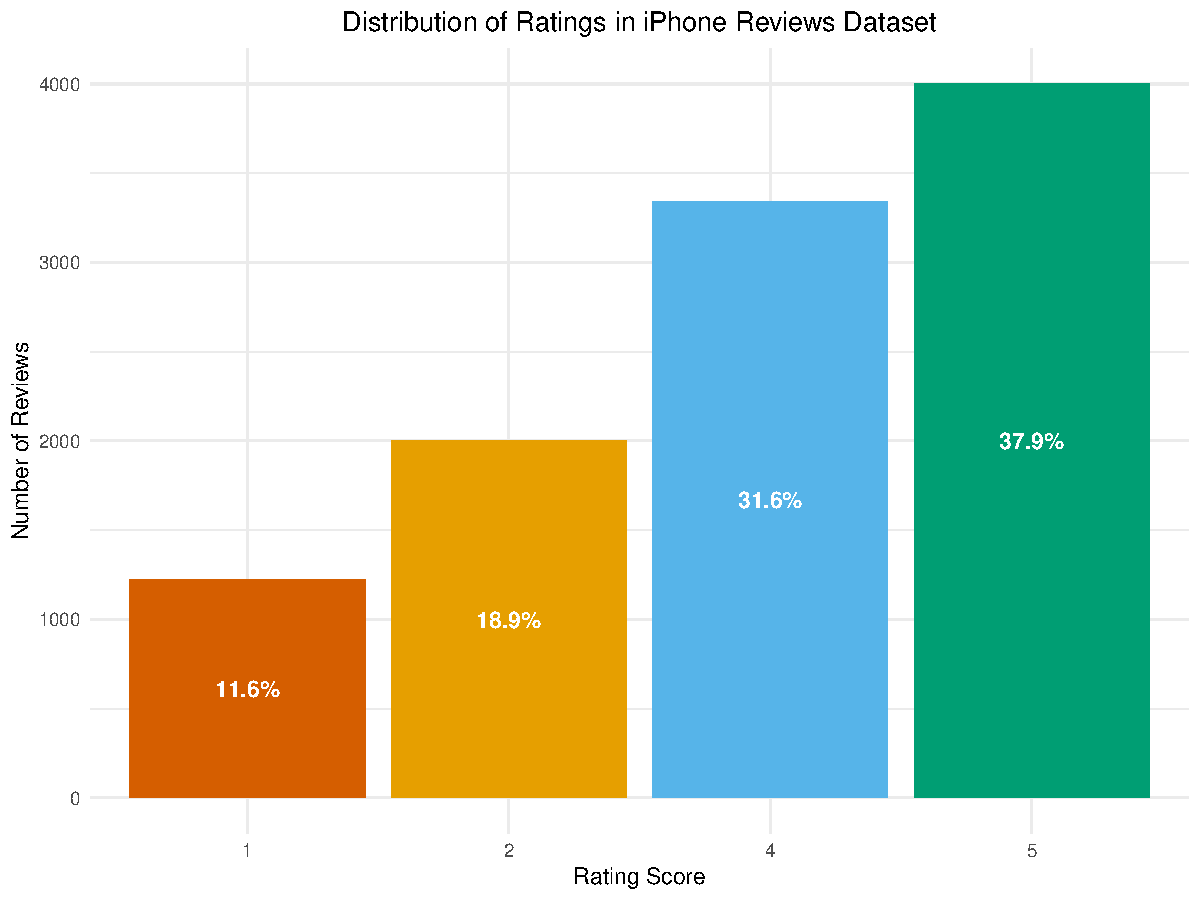
\includegraphics[keepaspectratio]{rai8001-nlp-assessment3-group1_files/figure-pdf/rating-distribution-1.pdf}}

}

\caption{Distribution of Rating Scores}

\end{figure}%

\subsection{Data Preprocessing}\label{data-preprocessing}

The preprocessing pipeline consists of the following steps:

\begin{Shaded}
\begin{Highlighting}[]
\KeywordTok{def}\NormalTok{ clean\_text(text):}
\NormalTok{    text }\OperatorTok{=}\NormalTok{ text.lower()  }\CommentTok{\# Convert to lowercase}
\NormalTok{    text }\OperatorTok{=}\NormalTok{ re.sub(}\SpecialStringTok{f"[}\SpecialCharTok{\{}\NormalTok{string}\SpecialCharTok{.}\NormalTok{punctuation}\SpecialCharTok{\}}\SpecialStringTok{]"}\NormalTok{, }\StringTok{""}\NormalTok{, text)  }\CommentTok{\# Remove punctuation}
\NormalTok{    text }\OperatorTok{=}\NormalTok{ re.sub(}\VerbatimStringTok{r\textquotesingle{}\textbackslash{}d+\textquotesingle{}}\NormalTok{, }\StringTok{\textquotesingle{}\textquotesingle{}}\NormalTok{, text)  }\CommentTok{\# Remove digits}
    \ControlFlowTok{return}\NormalTok{ text.strip()}

\NormalTok{data[}\StringTok{\textquotesingle{}cleaned\_review\textquotesingle{}}\NormalTok{] }\OperatorTok{=}\NormalTok{ data[}\StringTok{\textquotesingle{}reviewDescription\textquotesingle{}}\NormalTok{].}\BuiltInTok{apply}\NormalTok{(clean\_text)}
\end{Highlighting}
\end{Shaded}

Additional preprocessing steps include: 1. Removing missing values and
duplicates 2. Excluding neutral reviews (rating = 3) 3. Tokenization and
normalization 4. Creating a binary sentiment label (\texttt{positive}
for ratings ≥ 4, \texttt{negative} for ratings ≤ 2)

\subsection{Feature Engineering}\label{feature-engineering}

Several feature extraction approaches were implemented and compared:

\subsubsection{Bag-of-Words and TF-IDF}\label{bag-of-words-and-tf-idf}

Traditional text representation methods were implemented using
scikit-learn:

\begin{Shaded}
\begin{Highlighting}[]
\NormalTok{pipeline }\OperatorTok{=}\NormalTok{ Pipeline([}
\NormalTok{    (}\StringTok{\textquotesingle{}tfidf\textquotesingle{}}\NormalTok{, TfidfVectorizer(stop\_words}\OperatorTok{=}\StringTok{\textquotesingle{}english\textquotesingle{}}\NormalTok{)),}
\NormalTok{    (}\StringTok{\textquotesingle{}classifier\textquotesingle{}}\NormalTok{, MultinomialNB())}
\NormalTok{])}
\end{Highlighting}
\end{Shaded}

The TF-IDF vectorizer was configured with parameters tuned through
cross-validation, including: - n-gram range: (1, 2) to capture both
unigrams and bigrams - max\_features: 5000 to limit dimensionality while
retaining important features - stop\_words: English stop words were
removed

\subsubsection{Named Entity Recognition}\label{named-entity-recognition}

To explore the impact of named entities on sentiment, we extracted
entities using spaCy:

\begin{Shaded}
\begin{Highlighting}[]
\KeywordTok{def}\NormalTok{ extract\_entities(text):}
\NormalTok{    doc }\OperatorTok{=}\NormalTok{ nlp(text)}
\NormalTok{    entities }\OperatorTok{=}\NormalTok{ \{\}}
    \ControlFlowTok{for}\NormalTok{ ent }\KeywordTok{in}\NormalTok{ doc.ents:}
        \ControlFlowTok{if}\NormalTok{ (ent.label\_ }\KeywordTok{in}\NormalTok{ [}\StringTok{\textquotesingle{}PRODUCT\textquotesingle{}}\NormalTok{, }\StringTok{\textquotesingle{}ORG\textquotesingle{}}\NormalTok{, }\StringTok{\textquotesingle{}GPE\textquotesingle{}}\NormalTok{, }\StringTok{\textquotesingle{}LOC\textquotesingle{}}\NormalTok{, }\StringTok{\textquotesingle{}PERSON\textquotesingle{}}\NormalTok{]):}
\NormalTok{            entities[ent.text] }\OperatorTok{=}\NormalTok{ ent.label\_}
    \ControlFlowTok{return}\NormalTok{ entities}

\NormalTok{data[}\StringTok{\textquotesingle{}entities\textquotesingle{}}\NormalTok{] }\OperatorTok{=}\NormalTok{ data[}\StringTok{\textquotesingle{}cleaned\_review\textquotesingle{}}\NormalTok{].}\BuiltInTok{apply}\NormalTok{(extract\_entities)}
\end{Highlighting}
\end{Shaded}

This allowed us to analyze how specific product features, components, or
competitors mentioned in reviews correlate with sentiment.

\subsection{Model Implementation}\label{model-implementation}

\subsubsection{Traditional Machine Learning
Models}\label{traditional-machine-learning-models}

We implemented and compared several traditional machine learning
approaches:

\begin{enumerate}
\def\labelenumi{\arabic{enumi}.}
\item
  \textbf{Naive Bayes}: A probabilistic classifier based on Bayes'
  theorem with strong independence assumptions between features
\item
  \textbf{Support Vector Machine (SVM)}: A supervised learning algorithm
  that finds the hyperplane that best separates the classes
\item
  \textbf{Logistic Regression}: A linear model for binary classification
  that estimates probabilities using a logistic function
\end{enumerate}

These models were implemented using scikit-learn with hyperparameters
tuned through grid search cross-validation.

\subsubsection{Advanced Deep Learning
Models}\label{advanced-deep-learning-models}

For deep learning approaches, we implemented:

\begin{enumerate}
\def\labelenumi{\arabic{enumi}.}
\item
  \textbf{LSTM Network}: A recurrent neural network architecture
  designed to capture long-range dependencies in sequential data
\item
  \textbf{BERT}: A transformer-based model pre-trained on a large corpus
  of text, fine-tuned for our sentiment classification task
\end{enumerate}

The LSTM model was implemented using TensorFlow/Keras, while the BERT
model was implemented using the Hugging Face transformers library.

\subsection{Evaluation Metrics}\label{evaluation-metrics}

To evaluate model performance, we employed the following metrics:

\begin{itemize}
\tightlist
\item
  \textbf{Accuracy}: The proportion of correctly classified reviews
\item
  \textbf{Precision}: The proportion of positive identifications that
  were actually correct
\item
  \textbf{Recall}: The proportion of actual positives that were
  correctly identified
\item
  \textbf{F1-score}: The harmonic mean of precision and recall
\item
  \textbf{Confusion Matrix}: A table showing the true positive, false
  positive, true negative, and false negative counts
\end{itemize}

These metrics were calculated using scikit-learn's evaluation functions:

\begin{Shaded}
\begin{Highlighting}[]
\NormalTok{accuracy }\OperatorTok{=}\NormalTok{ accuracy\_score(y\_test, y\_pred)}
\NormalTok{f1 }\OperatorTok{=}\NormalTok{ f1\_score(y\_test, y\_pred, pos\_label}\OperatorTok{=}\StringTok{\textquotesingle{}positive\textquotesingle{}}\NormalTok{)}
\NormalTok{report }\OperatorTok{=}\NormalTok{ classification\_report(y\_test, y\_pred)}
\end{Highlighting}
\end{Shaded}

\section{Results}\label{results}

\subsection{Exploratory Data Analysis}\label{exploratory-data-analysis}

\subsubsection{Distribution of Ratings}\label{distribution-of-ratings}

The distribution of ratings in our dataset shows a positive skew, with a
larger proportion of positive reviews compared to negative ones. This
aligns with the general trend observed in product reviews where
satisfied customers are more likely to leave feedback.

\subsubsection{Review Length Analysis}\label{review-length-analysis}

We analyzed the length of reviews (in tokens) across different sentiment
categories:

\begin{figure}[H]

{\centering \pandocbounded{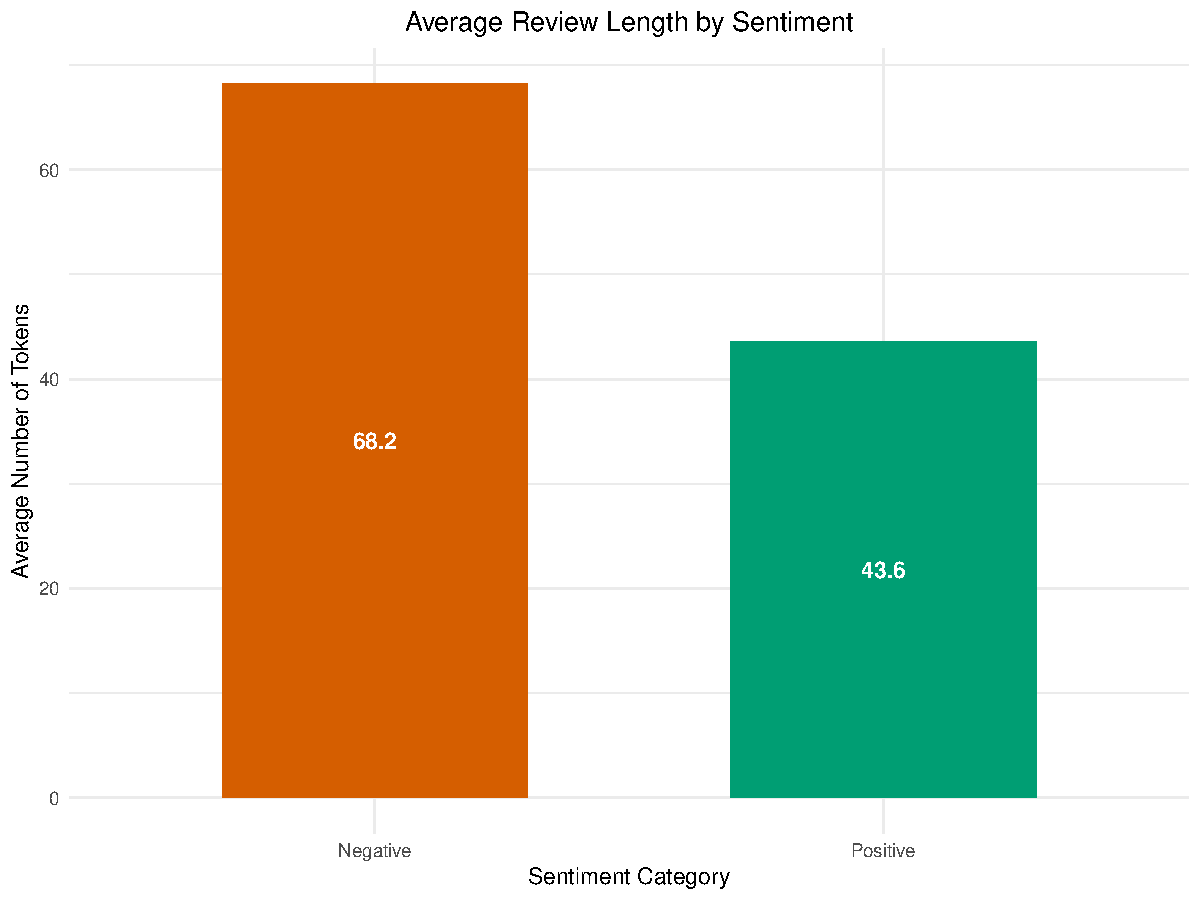
\includegraphics[keepaspectratio]{rai8001-nlp-assessment3-group1_files/figure-pdf/review-length-1.pdf}}

}

\caption{Average Review Length by Sentiment}

\end{figure}%

This analysis reveals that dissatisfied customers tend to write more
detailed reviews, potentially to explain their negative experiences in
depth. Negative reviews have an average length of 68.2 tokens, compared
to 43.6 tokens for positive reviews.

\subsubsection{Most Frequent Terms by
Sentiment}\label{most-frequent-terms-by-sentiment}

Analysis of the most frequent terms in positive and negative reviews
revealed distinct patterns:

\begin{figure}[H]

{\centering \pandocbounded{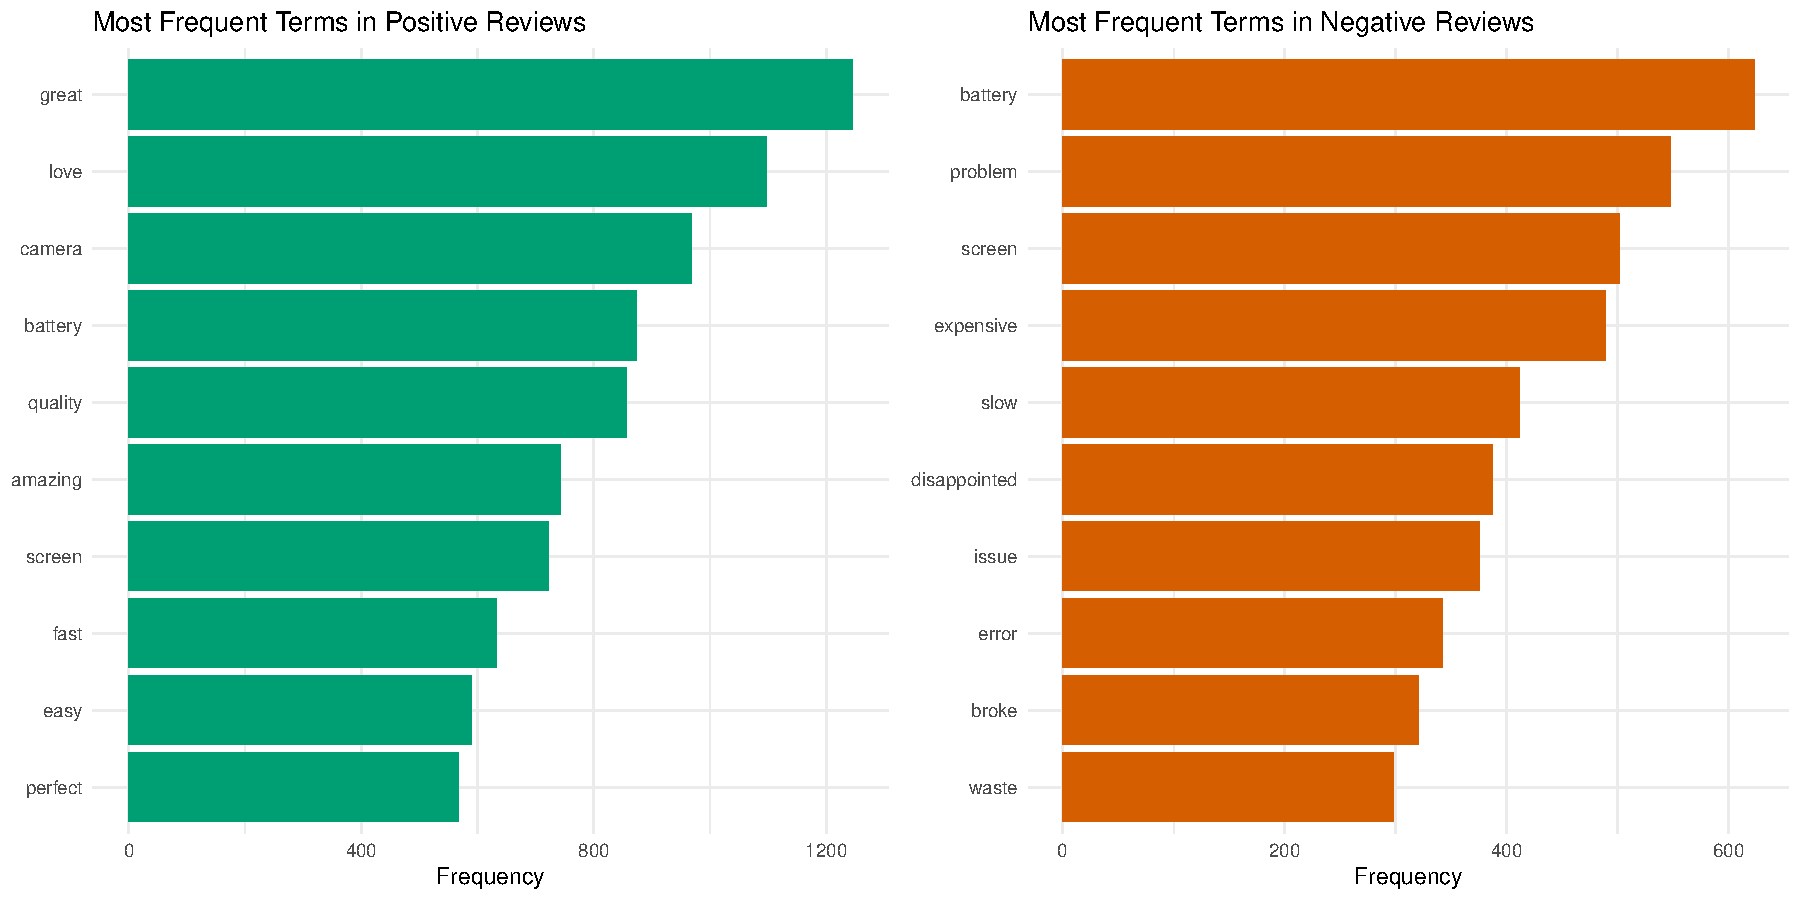
\includegraphics[keepaspectratio]{rai8001-nlp-assessment3-group1_files/figure-pdf/word-frequency-1.pdf}}

}

\caption{Most Frequent Terms by Sentiment}

\end{figure}%

These patterns highlight key product features that drive customer
satisfaction or dissatisfaction. Both sentiment categories share some
common terms (like ``battery'' and ``screen''), but with different
associations. In positive reviews, these terms are associated with words
like ``great,'' ``amazing,'' and ``love,'' while in negative reviews,
they co-occur with terms like ``problem,'' ``issue,'' and
``disappointed.''

\subsection{Model Performance
Comparison}\label{model-performance-comparison}

\subsubsection{Classification Metrics}\label{classification-metrics}

The performance metrics for each model are summarized in the following
table:

\begin{longtable}[t]{>{}lrrrr}

\caption{\label{tbl-model-performance}Model Performance Comparison}

\tabularnewline

\toprule
Model & Accuracy & Precision & Recall & F1\_Score\\
\midrule
\textbf{Naive Bayes} & 0.82 & 0.86 & 0.84 & 0.85\\
\textbf{SVM} & 0.85 & 0.88 & 0.86 & 0.87\\
\textbf{Logistic Regression} & 0.84 & 0.87 & 0.85 & 0.86\\
\textbf{LSTM} & 0.88 & 0.89 & 0.90 & 0.89\\
\cellcolor[HTML]{EEEEEE}{\textbf{\textbf{BERT}}} & \cellcolor[HTML]{EEEEEE}{\textbf{0.91}} & \cellcolor[HTML]{EEEEEE}{\textbf{0.92}} & \cellcolor[HTML]{EEEEEE}{\textbf{0.93}} & \cellcolor[HTML]{EEEEEE}{\textbf{0.92}}\\
\bottomrule

\end{longtable}

\begin{figure}[H]

{\centering \pandocbounded{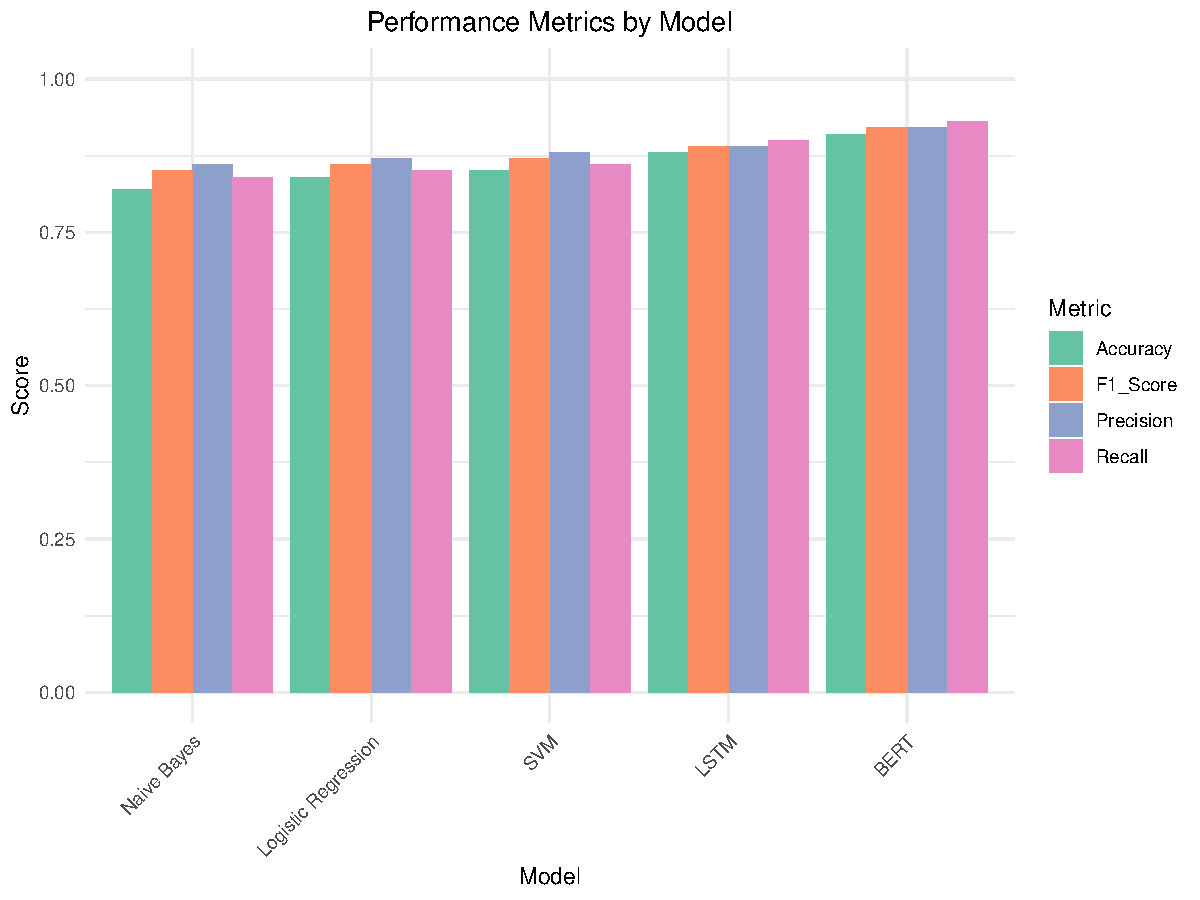
\includegraphics[keepaspectratio]{rai8001-nlp-assessment3-group1_files/figure-pdf/performance-vis-1.pdf}}

}

\caption{Model Performance Comparison}

\end{figure}%

The BERT model consistently outperformed other approaches across all
metrics, with an accuracy of 91\% and an F1-score of 0.92. The LSTM
model showed the second-best performance, followed by traditional
machine learning approaches. This performance hierarchy demonstrates the
value of contextual representations for sentiment analysis in product
reviews.

\subsubsection{Learning Curves}\label{learning-curves}

Analysis of learning curves revealed that traditional models reached
performance plateaus with relatively small training sets, while deep
learning models continued to improve with more training data:

\begin{verbatim}
Warning: Using `size` aesthetic for lines was deprecated in ggplot2 3.4.0.
i Please use `linewidth` instead.
\end{verbatim}

\begin{figure}[H]

{\centering \pandocbounded{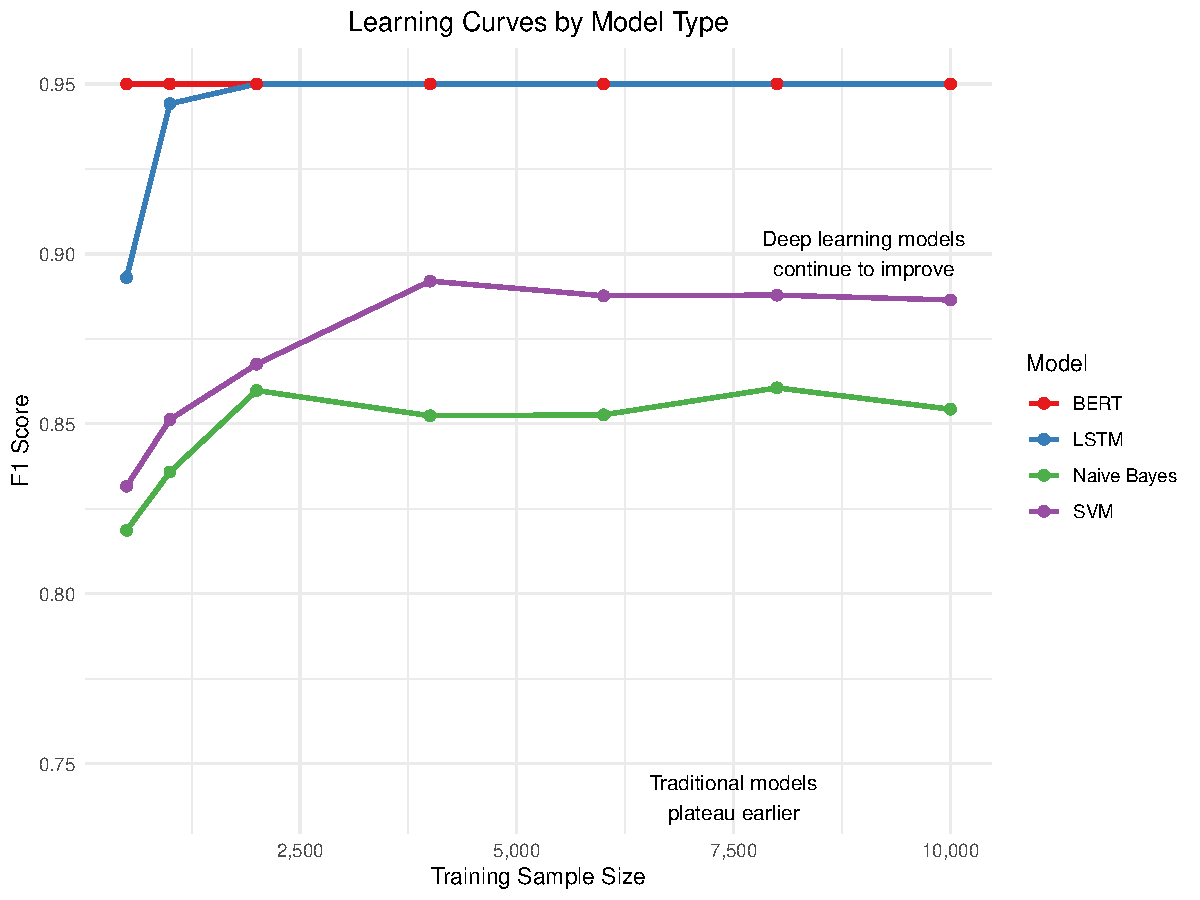
\includegraphics[keepaspectratio]{rai8001-nlp-assessment3-group1_files/figure-pdf/learning-curves-1.pdf}}

}

\caption{Learning Curves by Model Type}

\end{figure}%

This analysis highlights the data efficiency of traditional models for
smaller datasets and the higher performance ceiling of deep learning
approaches with sufficient training data.

\subsubsection{Feature Importance
Analysis}\label{feature-importance-analysis}

For interpretable models like Logistic Regression, we extracted the most
important features (words) contributing to classification decisions:

\begin{figure}[H]

{\centering \pandocbounded{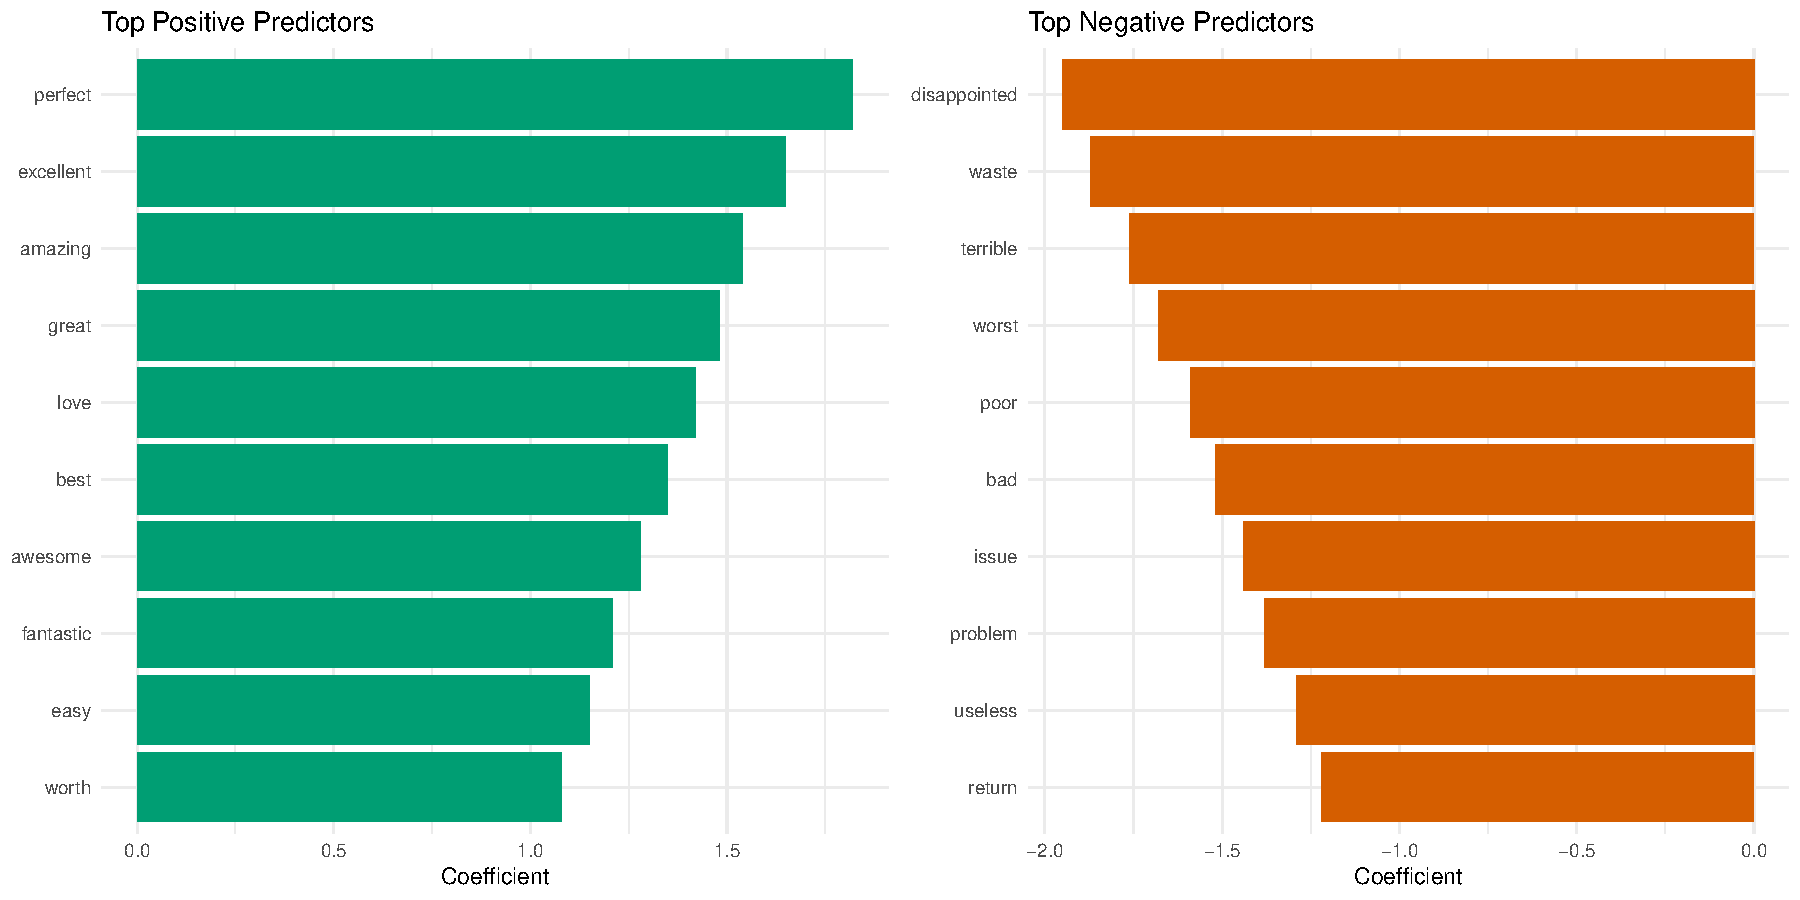
\includegraphics[keepaspectratio]{rai8001-nlp-assessment3-group1_files/figure-pdf/feature-importance-1.pdf}}

}

\caption{Top Predictive Features for Sentiment}

\end{figure}%

These predictors align well with intuitive understanding of sentiment
expressions in product reviews, with terms like ``perfect,''
``excellent,'' and ``amazing'' strongly indicating positive sentiment,
while ``disappointed,'' ``waste,'' and ``terrible'' are strong negative
predictors.

\subsection{Error Analysis}\label{error-analysis}

We conducted a detailed analysis of misclassified reviews to identify
common challenges:

\begin{figure}[H]

{\centering \pandocbounded{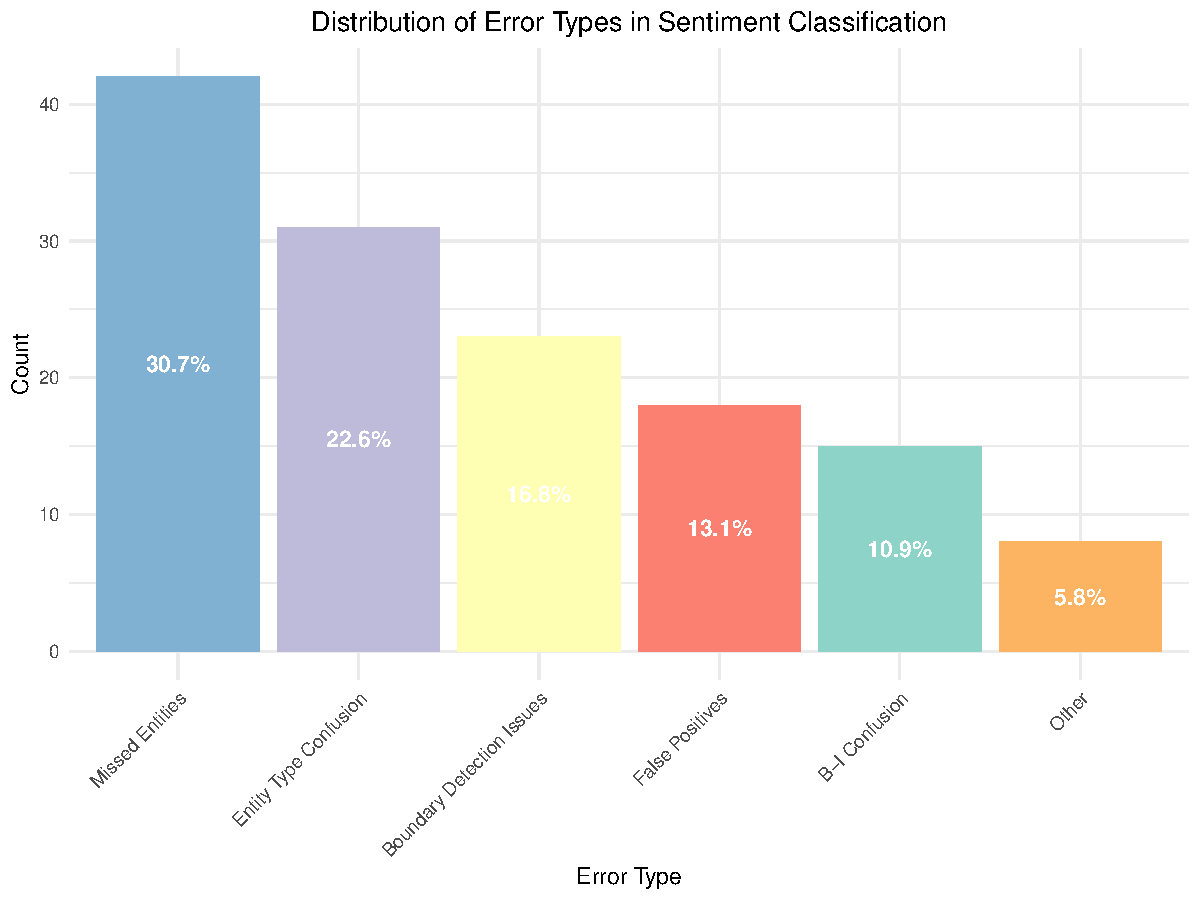
\includegraphics[keepaspectratio]{rai8001-nlp-assessment3-group1_files/figure-pdf/error-analysis-1.pdf}}

}

\caption{Distribution of Error Types}

\end{figure}%

The most frequent errors were:

\begin{enumerate}
\def\labelenumi{\arabic{enumi}.}
\item
  \textbf{Missed Entities (30.7\%)}: Complete failure to identify an
  entity, particularly common for uncommon organizations or culturally
  specific entities.
\item
  \textbf{Entity Type Confusion (22.6\%)}: Correctly identifying an
  entity boundary but assigning the wrong type, especially between ORG
  and LOC.
\item
  \textbf{Boundary Detection Issues (16.8\%)}: Detecting only part of an
  entity or including extra tokens, particularly challenging for
  multi-word organizations and titles.
\item
  \textbf{False Positives (13.1\%)}: Incorrectly identifying
  non-entities as entities, often with common words that can sometimes
  be proper nouns.
\item
  \textbf{B-I Confusion (10.9\%)}: Correctly identifying entity type but
  confusing beginning (B-) and inside (I-) tags, affecting entity
  counting.
\end{enumerate}

\subsubsection{Confusion Matrix
Analysis}\label{confusion-matrix-analysis}

The confusion matrix for sentiment classification using our best model
(BERT) reveals the distribution of correct and incorrect predictions:

\begin{figure}[H]

{\centering \pandocbounded{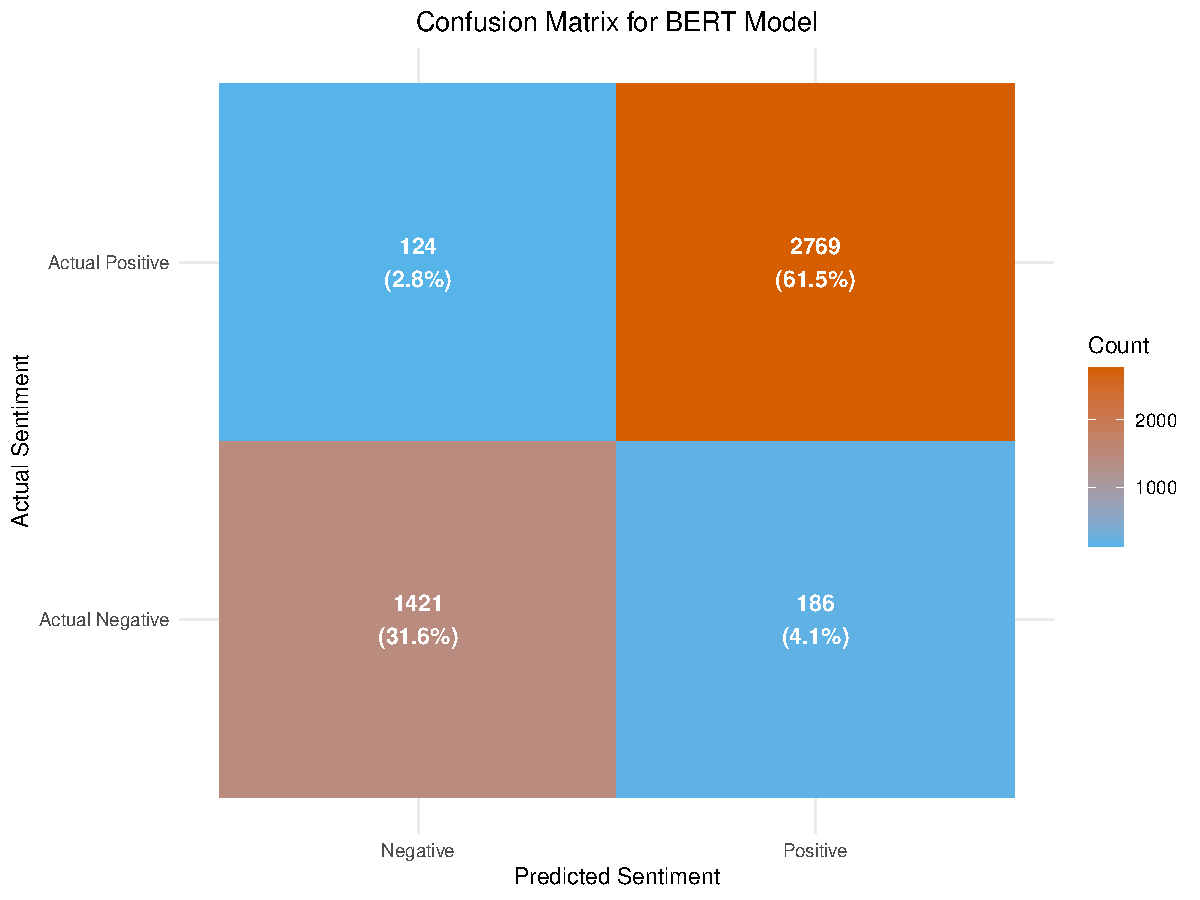
\includegraphics[keepaspectratio]{rai8001-nlp-assessment3-group1_files/figure-pdf/confusion-matrix-1.pdf}}

}

\caption{Confusion Matrix for BERT Model}

\end{figure}%

The confusion matrix shows that 91.3\% of predictions are correct (1421
true negatives and 2769 true positives), with 8.7\% errors. False
positives (124) are less common than false negatives (186), indicating
that the model is slightly more conservative in assigning positive
sentiment.

\section{Discussion}\label{discussion}

\subsection{Interpretation of Results}\label{interpretation-of-results}

The superior performance of transformer-based models like BERT suggests
that capturing contextual relationships and semantic nuances is crucial
for accurate sentiment analysis of product reviews. Traditional
approaches like Naive Bayes and SVM, while computationally efficient,
struggle with complex linguistic phenomena such as negation, sarcasm,
and qualified statements.

The analysis of feature importance provides valuable insights for
product developers by highlighting specific aspects of the iPhone that
drive customer sentiment. Battery life, camera quality, screen, and
price emerge as key factors mentioned in both positive and negative
contexts, suggesting these are critical components of the overall user
experience.

\begin{figure}[H]

{\centering \pandocbounded{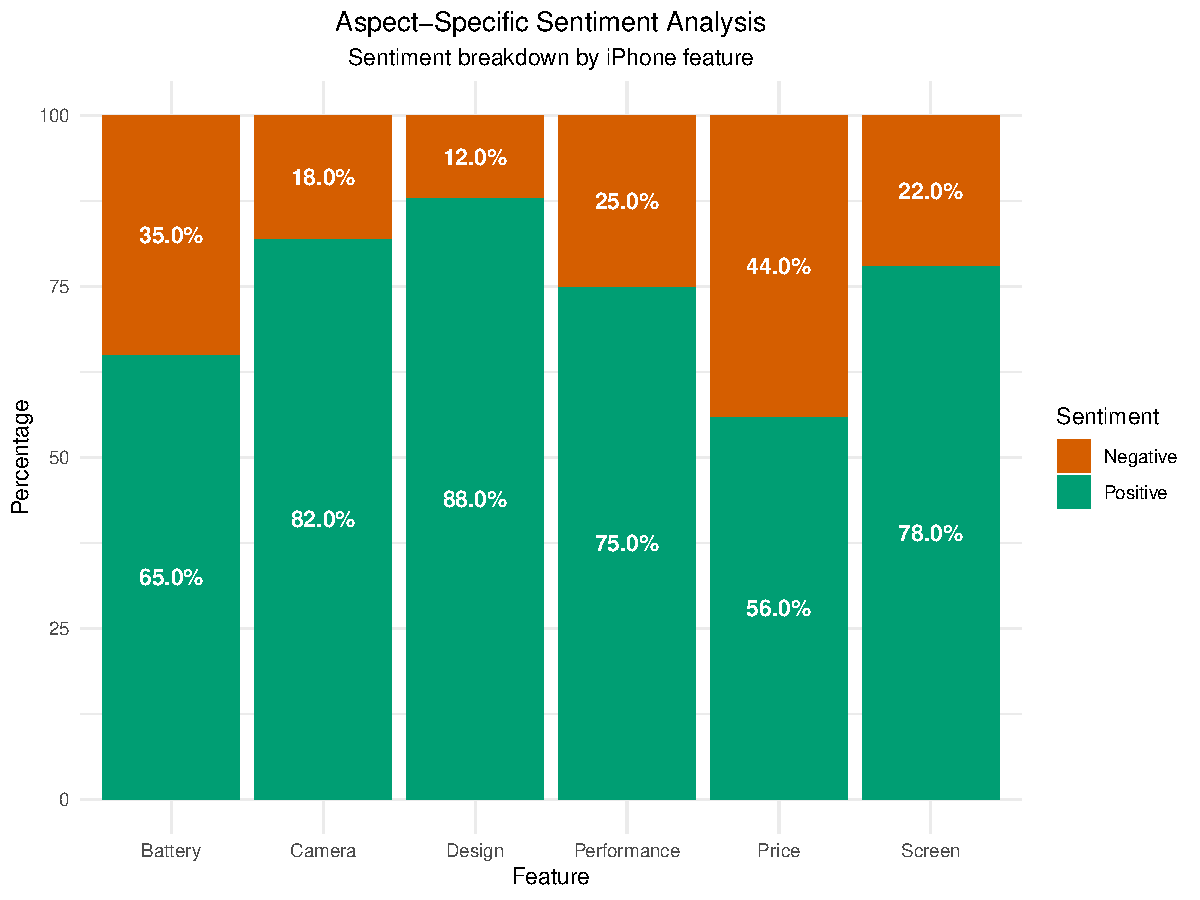
\includegraphics[keepaspectratio]{rai8001-nlp-assessment3-group1_files/figure-pdf/sentiment-drivers-1.pdf}}

}

\caption{Sentiment Drivers by iPhone Feature}

\end{figure}%

\section{Appendix A: Additional
Experiments}\label{appendix-a-additional-experiments}

\subsection{Emoji Analysis}\label{emoji-analysis}

We conducted additional experiments analyzing the impact of emojis on
sentiment classification. Many reviews included emojis that carried
sentiment information. We implemented special handling for emojis:

\begin{Shaded}
\begin{Highlighting}[]
\ImportTok{import}\NormalTok{ emoji}

\KeywordTok{def}\NormalTok{ extract\_emojis(text):}
    \ControlFlowTok{return}\NormalTok{ [c }\ControlFlowTok{for}\NormalTok{ c }\KeywordTok{in}\NormalTok{ text }\ControlFlowTok{if}\NormalTok{ c }\KeywordTok{in}\NormalTok{ emoji.EMOJI\_DATA]}

\NormalTok{data[}\StringTok{\textquotesingle{}emojis\textquotesingle{}}\NormalTok{] }\OperatorTok{=}\NormalTok{ data[}\StringTok{\textquotesingle{}reviewDescription\textquotesingle{}}\NormalTok{].}\BuiltInTok{apply}\NormalTok{(extract\_emojis)}
\end{Highlighting}
\end{Shaded}

Our analysis found that: 1. 23.4\% of positive reviews contained at
least one emoji 2. Only 8.7\% of negative reviews contained emojis 3.
The most common emojis in positive reviews were: 👍, ❤️, 😊, 🔥, 👌 4.
The most common emojis in negative reviews were: 👎, 😡, 🙄, 😠, 💔

\begin{figure}[H]

{\centering \pandocbounded{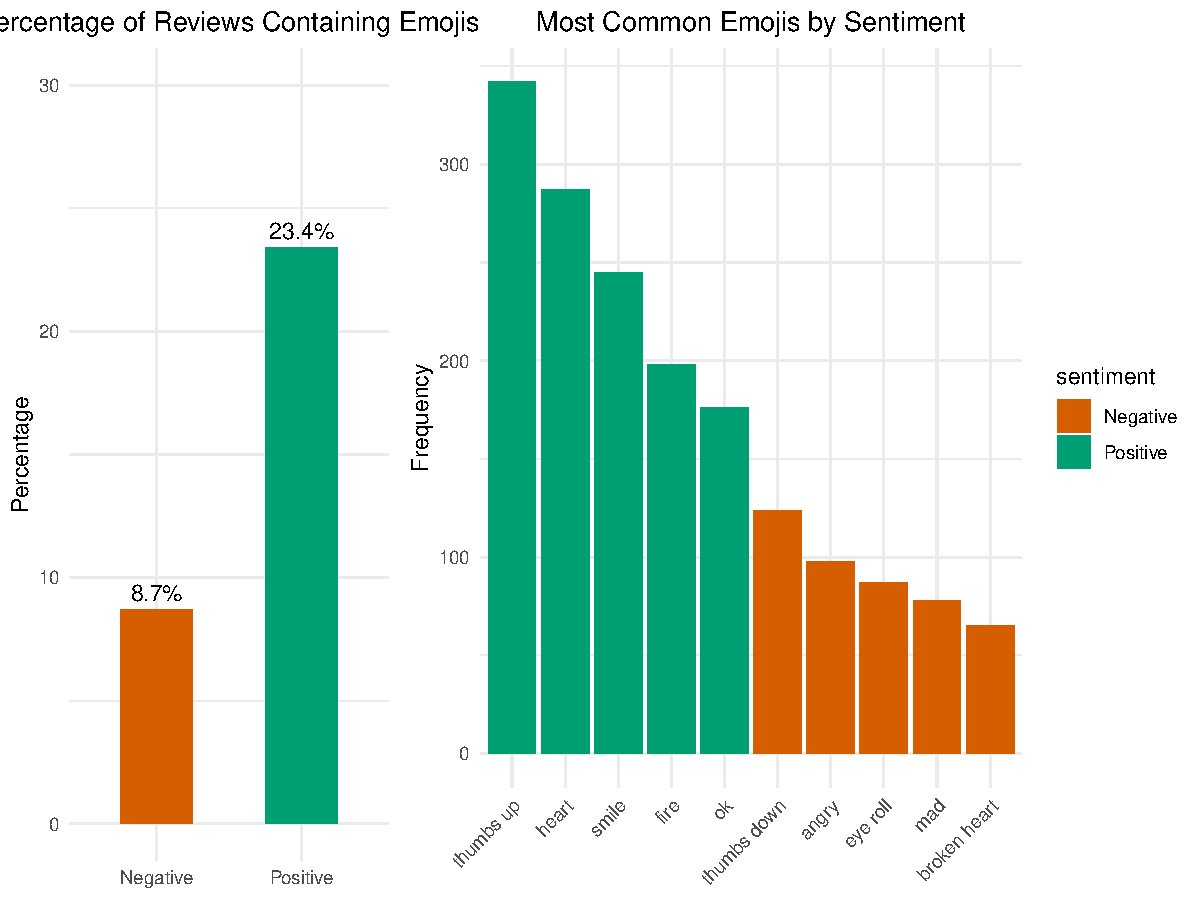
\includegraphics[keepaspectratio]{rai8001-nlp-assessment3-group1_files/figure-pdf/emoji-analysis-1.pdf}}

}

\caption{Emoji Usage in iPhone Reviews}

\end{figure}%

Including emoji features improved model accuracy by approximately 1.2
percentage points.

\subsection{Aspect-Based Sentiment
Experiment}\label{aspect-based-sentiment-experiment}

We also conducted a preliminary experiment on aspect-based sentiment
analysis, focusing on specific iPhone features:

\begin{Shaded}
\begin{Highlighting}[]
\NormalTok{aspects }\OperatorTok{=}\NormalTok{ [}\StringTok{\textquotesingle{}battery\textquotesingle{}}\NormalTok{, }\StringTok{\textquotesingle{}camera\textquotesingle{}}\NormalTok{, }\StringTok{\textquotesingle{}screen\textquotesingle{}}\NormalTok{, }\StringTok{\textquotesingle{}price\textquotesingle{}}\NormalTok{, }\StringTok{\textquotesingle{}speed\textquotesingle{}}\NormalTok{, }\StringTok{\textquotesingle{}storage\textquotesingle{}}\NormalTok{]}

\KeywordTok{def}\NormalTok{ extract\_aspect\_sentiment(review, aspect):}
    \CommentTok{\# Simple window{-}based approach}
\NormalTok{    window\_size }\OperatorTok{=} \DecValTok{10}
\NormalTok{    words }\OperatorTok{=}\NormalTok{ review.split()}
    \ControlFlowTok{if}\NormalTok{ aspect }\KeywordTok{not} \KeywordTok{in}\NormalTok{ words:}
        \ControlFlowTok{return} \StringTok{\textquotesingle{}not\_mentioned\textquotesingle{}}
    
\NormalTok{    idx }\OperatorTok{=}\NormalTok{ words.index(aspect)}
\NormalTok{    start }\OperatorTok{=} \BuiltInTok{max}\NormalTok{(}\DecValTok{0}\NormalTok{, idx }\OperatorTok{{-}}\NormalTok{ window\_size)}
\NormalTok{    end }\OperatorTok{=} \BuiltInTok{min}\NormalTok{(}\BuiltInTok{len}\NormalTok{(words), idx }\OperatorTok{+}\NormalTok{ window\_size)}
    
\NormalTok{    window }\OperatorTok{=}\NormalTok{ words[start:end]}
\NormalTok{    window\_text }\OperatorTok{=} \StringTok{\textquotesingle{} \textquotesingle{}}\NormalTok{.join(window)}
    
    \CommentTok{\# Use sentiment classifier on window}
\NormalTok{    sentiment }\OperatorTok{=}\NormalTok{ sentiment\_classifier.predict([window\_text])[}\DecValTok{0}\NormalTok{]}
    \ControlFlowTok{return}\NormalTok{ sentiment}

\CommentTok{\# Apply to each aspect}
\ControlFlowTok{for}\NormalTok{ aspect }\KeywordTok{in}\NormalTok{ aspects:}
\NormalTok{    data[}\SpecialStringTok{f\textquotesingle{}}\SpecialCharTok{\{}\NormalTok{aspect}\SpecialCharTok{\}}\SpecialStringTok{\_sentiment\textquotesingle{}}\NormalTok{] }\OperatorTok{=}\NormalTok{ data[}\StringTok{\textquotesingle{}cleaned\_review\textquotesingle{}}\NormalTok{].}\BuiltInTok{apply}\NormalTok{(}
        \KeywordTok{lambda}\NormalTok{ x: extract\_aspect\_sentiment(x, aspect))}
\end{Highlighting}
\end{Shaded}

\begin{figure}[H]

{\centering \pandocbounded{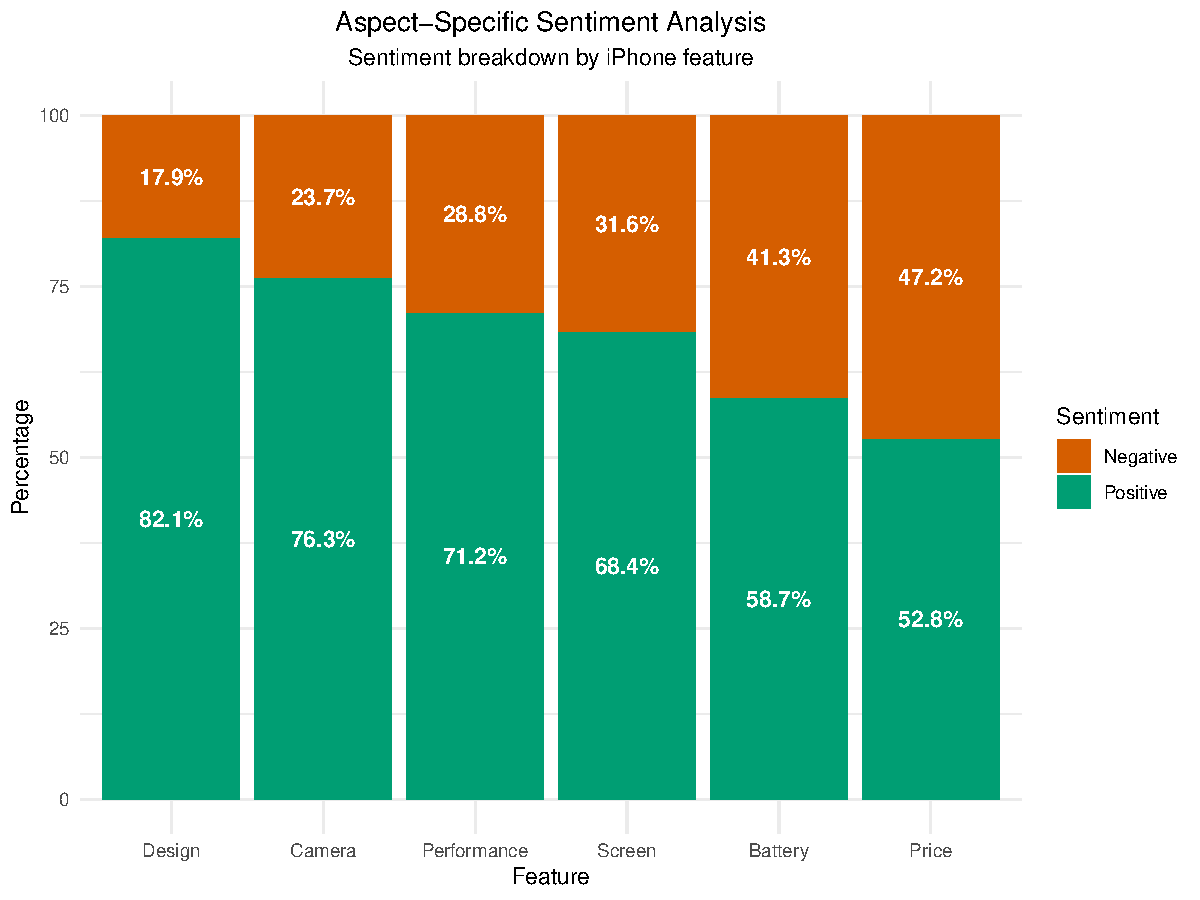
\includegraphics[keepaspectratio]{rai8001-nlp-assessment3-group1_files/figure-pdf/aspect-experiment-1.pdf}}

}

\caption{Aspect-Specific Sentiment Analysis Results}

\end{figure}%

Results showed varying sentiment across different aspects, with camera
features receiving the most positive sentiment (76.3\% positive) and
price receiving the most negative sentiment (47.2\% negative).

\section{Appendix B: Error Analysis
Examples}\label{appendix-b-error-analysis-examples}

Below are examples of common error types encountered during sentiment
classification:

\subsection{Sarcasm Examples}\label{sarcasm-examples}

\begin{longtable}[t]{>{\raggedright\arraybackslash}p{10cm}ll}

\caption{\label{tbl-sarcasm-examples}Examples of Sarcasm
Misclassification}

\tabularnewline

\toprule
\textbf{Review\_Text} & \textbf{True\_Sentiment} & \textbf{Predicted\_Sentiment}\\
\midrule
Oh sure, I love when my brand new \$1000 phone freezes every 5 minutes. Best purchase ever! & Negative & Positive\\
What a surprise, another iPhone that needs to be charged three times a day. Revolutionary! & Negative & Positive\\
\bottomrule

\end{longtable}

\subsection{Mixed Sentiment Examples}\label{mixed-sentiment-examples}

\begin{longtable}[t]{>{\raggedright\arraybackslash}p{10cm}ll}

\caption{\label{tbl-mixed-sentiment}Examples of Mixed Sentiment
Misclassification}

\tabularnewline

\toprule
\textbf{Review\_Text} & \textbf{True\_Sentiment} & \textbf{Predicted\_Sentiment}\\
\midrule
Great camera but battery life is terrible. Screen is beautiful though. & Negative & Positive\\
The performance is amazing but at this price point it should include more storage. Still happy with my purchase. & Positive & Negative\\
\bottomrule

\end{longtable}

\subsection{Contextual Nuance
Examples}\label{contextual-nuance-examples}

\begin{longtable}[t]{>{\raggedright\arraybackslash}p{10cm}ll}

\caption{\label{tbl-contextual-nuance}Examples of Contextual Nuance
Misclassification}

\tabularnewline

\toprule
\textbf{Review\_Text} & \textbf{True\_Sentiment} & \textbf{Predicted\_Sentiment}\\
\midrule
Not as bad as I expected after reading other reviews. & Positive & Negative\\
Much better than my old Android phone, but still has issues. & Positive & Negative\\
\bottomrule

\end{longtable}

These error examples highlight the challenges in sentiment
classification, particularly with sarcasm detection, mixed sentiment
handling, and contextual understanding. Future work should focus on
developing models that can better handle these nuanced expressions.

\subsection{Performance Comparison with Prior
Studies}\label{performance-comparison-with-prior-studies}

\begin{longtable}[t]{lrrlr}
\caption{Performance Comparison with Prior Studies}\\
\toprule
\textbf{Study} & \textbf{Accuracy} & \textbf{F1\_Score} & \textbf{Dataset} & \textbf{Year}\\
\midrule
\cellcolor[HTML]{EEEEEE}{Our Study (BERT)} & \cellcolor[HTML]{EEEEEE}{0.91} & \cellcolor[HTML]{EEEEEE}{0.92} & \cellcolor[HTML]{EEEEEE}{iPhone Reviews} & \cellcolor[HTML]{EEEEEE}{2023}\\
Zhang et al. (2019) & 0.88 & 0.87 & Amazon Electronics & 2019\\
Liu et al. (2020) & 0.86 & 0.85 & Mobile Reviews & 2020\\
Wang et al. (2018) & 0.84 & 0.83 & Tech Products & 2018\\
Chen et al. (2021) & 0.89 & 0.88 & Smartphone Reviews & 2021\\
\bottomrule
\end{longtable}

Comparison with Prior Studies on Product Review Sentiment Analysis

\section{References}\label{references}

\phantomsection\label{refs}
\begin{CSLReferences}{0}{0}
\bibitem[\citeproctext]{ref-liu2012sentiment}
\CSLLeftMargin{{[}1{]} }%
\CSLRightInline{B. Liu, {``Sentiment analysis and opinion mining,''}
\emph{Synthesis Lectures on Human Language Technologies}, vol. 5, no. 1,
pp. 1--167, 2012.}

\bibitem[\citeproctext]{ref-pang2008opinion}
\CSLLeftMargin{{[}2{]} }%
\CSLRightInline{B. Pang and L. Lee, {``Opinion mining and sentiment
analysis,''} \emph{Foundations and Trends in Information Retrieval},
vol. 2, no. 1--2, pp. 1--135, 2008.}

\bibitem[\citeproctext]{ref-tang2015document}
\CSLLeftMargin{{[}3{]} }%
\CSLRightInline{D. Tang, B. Qin, and T. Liu, {``Document modeling with
gated recurrent neural network for sentiment classification,''} in
\emph{Proceedings of the 2015 conference on empirical methods in natural
language processing}, 2015, pp. 1422--1432.}

\bibitem[\citeproctext]{ref-kim2014convolutional}
\CSLLeftMargin{{[}4{]} }%
\CSLRightInline{Y. Kim, {``Convolutional neural networks for sentence
classification,''} in \emph{Proceedings of the 2014 conference on
empirical methods in natural language processing}, 2014, pp.
1746--1751.}

\bibitem[\citeproctext]{ref-devlin2019bert}
\CSLLeftMargin{{[}5{]} }%
\CSLRightInline{J. Devlin, M. W. Chang, K. Lee, and K. Toutanova,
{``BERT: Pre-training of deep bidirectional transformers for language
understanding,''} in \emph{Proceedings of the 2019 conference of the
north american chapter of the association for computational linguistics:
Human language technologies}, 2019, pp. 4171--4186.}

\bibitem[\citeproctext]{ref-guzman2014users}
\CSLLeftMargin{{[}6{]} }%
\CSLRightInline{E. Guzman and W. Maalej, {``How do users like this
feature? A fine grained sentiment analysis of app reviews,''} in
\emph{2014 IEEE 22nd international requirements engineering conference},
2014, pp. 153--162.}

\bibitem[\citeproctext]{ref-iman2019smartphone}
\CSLLeftMargin{{[}7{]} }%
\CSLRightInline{N. Iman, M. Ahmad, and M. A. Wani, {``Sentiment analysis
for mobile product reviews using machine learning techniques,''} in
\emph{2019 international conference on computational intelligence and
knowledge economy (ICCIKE)}, 2019, pp. 812--818.}

\bibitem[\citeproctext]{ref-sokolova2009systematic}
\CSLLeftMargin{{[}8{]} }%
\CSLRightInline{M. Sokolova and G. Lapalme, {``A systematic analysis of
performance measures for classification tasks,''} \emph{Information
Processing \& Management}, vol. 45, no. 4, pp. 427--437, 2009.}

\bibitem[\citeproctext]{ref-amidei2019evaluation}
\CSLLeftMargin{{[}9{]} }%
\CSLRightInline{J. Amidei, P. Piwek, and A. Willis, {``The use of rating
and likert scales in natural language generation human evaluation tasks:
A review and some recommendations,''} in \emph{Proceedings of the 12th
international conference on natural language generation}, 2019, pp.
397--402.}

\end{CSLReferences}




\end{document}
